\documentclass[a4paper]{article}
\usepackage[spanish]{babel}
\usepackage[utf8]{inputenc}
\usepackage{charter}   % tipografia
\usepackage{graphicx}
\usepackage{courier}
%\usepackage{makeidx}
\usepackage{paralist} %itemize inline
\usepackage{caption}
%\usepackage{float}
%\usepackage{amsmath, amsthm, amssymb}
%\usepackage{amsfonts}
%\usepackage{sectsty}
%\usepackage{charter}
%\usepackage{wrapfig}
%\usepackage{listings}
%\lstset{language=C}
\usepackage{booktabs}

\usepackage{color} % para snipets de codigo coloreados
\usepackage{fancybox}  % para el sbox de los snipets de codigo

\definecolor{litegrey}{gray}{0.94}

% \newenvironment{sidebar}{%
% 	\begin{Sbox}\begin{minipage}{.85\textwidth}}%
% 	{\end{minipage}\end{Sbox}%
% 		\begin{center}\setlength{\fboxsep}{6pt}%
% 		\shadowbox{\TheSbox}\end{center}}
% \newenvironment{warning}{%
% 	\begin{Sbox}\begin{minipage}{.85\textwidth}\sffamily\lite\small\RaggedRight}%
% 	{\end{minipage}\end{Sbox}%
% 		\begin{center}\setlength{\fboxsep}{6pt}%
% 		\colorbox{litegrey}{\TheSbox}\end{center}}

\newenvironment{codesnippet}{%
	\begin{Sbox}\begin{minipage}{\textwidth}\sffamily\small}%
	{\end{minipage}\end{Sbox}%
		\begin{center}%
		\vspace{-0.4cm}\colorbox{litegrey}{\TheSbox}\end{center}\vspace{0.3cm}}



\usepackage{fancyhdr}
\pagestyle{fancy}

%\renewcommand{\chaptermark}[1]{\markboth{#1}{}}
\renewcommand{\sectionmark}[1]{\markright{\thesection\ - #1}}

\fancyhf{}

\fancyhead[LO]{Sección \rightmark} % \thesection\ 
\fancyfoot[LO]{\small{Nombre Apellido, Nombre Apellido, Nombre Apellido}}
\fancyfoot[RO]{\thepage}
\renewcommand{\headrulewidth}{0.5pt}
\renewcommand{\footrulewidth}{0.5pt}
\setlength{\hoffset}{-0.8in}
\setlength{\textwidth}{16cm}
%\setlength{\hoffset}{-1.1cm}
%\setlength{\textwidth}{16cm}
\setlength{\headsep}{0.5cm}
\setlength{\textheight}{25cm}
\setlength{\voffset}{-0.7in}
\setlength{\headwidth}{\textwidth}
\setlength{\headheight}{13.1pt}

\renewcommand{\baselinestretch}{1.1}  % line spacing


% \setcounter{secnumdepth}{2}
\usepackage{underscore}
\usepackage{caratula}
\usepackage{url}

% ******************************************************** %
%              TEMPLATE DE INFORME ORGA2 v0.1              %
% ******************************************************** %
% ******************************************************** %
%                                                          %
% ALGUNOS PAQUETES REQUERIDOS (EN UBUNTU):                 %
% ========================================
%                                                          %
% texlive-latex-base                                       %
% texlive-latex-recommended                                %
% texlive-fonts-recommended                                %
% texlive-latex-extra?                                     %
% texlive-lang-spanish (en ubuntu 13.10)                   %
% ******************************************************** %



\begin{document}


\thispagestyle{empty}
\materia{Organización del Computador II}
\submateria{Segundo Cuatrimestre de 2014}
\titulo{Trabajo Práctico III}
\subtitulo{System Programming-Zombi Defense}
\integrante{Christian Chibana}{586/13}{christian.chiba93@gmail.com}
\integrante{Javier Minces Müller}{231/13}{javijavi1994@hotmail.com}
\integrante{Nicolás Roulet}{587/13}{nicoroulet@gmail.com}

\maketitle
\newpage

\thispagestyle{empty}
\vfill
\begin{abstract}

\end{abstract}

\thispagestyle{empty}
\vspace{3cm}
\tableofcontents
\newpage


%\normalsize
\newpage



\section{Introducción}
El objetivo del siguiente trabajo práctico es explorar los conceptos fundamentales de la programación de sistemas, desarrollando para tal fin un sistema con capacidad de manejo de múltiples tareas de manera dinámica y una interfaz de comunicación con el usuario. 

La base del sistema consiste en un kernel provisto de estructuras de datos que pe permiten administrar memoria con diferentes niveles de privilegio, capturar eventuales errores en tiempo de ejecución a fin de actuar consecuentemente y recibir interrupciones de dispositivos externos para permitir la entrada de datos. A su vez, está diseñado para poder conmutar tareas a fin de simular una ejecución simultánea.

Estas herramientas permiten implementar un juego de dos jugadores donde cada uno tiene a su disposición zombis (tareas) con los que combatir a su contrincante.

Esta es la estructura de los archivos:

\smallskip
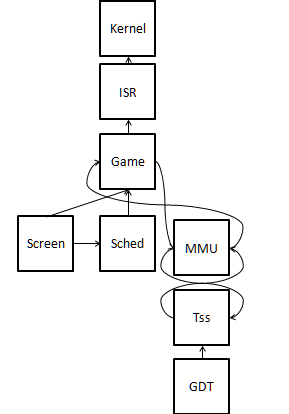
\includegraphics{imagenes/Includes.png}

\section{Global Descriptor Table (GDT)}
La Global Descriptor Table (GDT) es una estructura de datos que permite almacenar descriptores de los diferentes segmentos del sistema. Contiene por convención un descriptor nulo en la primer entrada. En este caso particular, las siguientes 7 entradas se consideran reservadas, por lo que los descriptores utilizados comienzan a partir de la posición 8.

La administración de memoria se basa en cuatro segmentos principales:
\begin{itemize}
\item Segmento de código de nivel 0: será utilizado para ejecutar las instrucciones del kernel y demás rutinas que requieran nivel de supervisor.
\item Segmento de datos de nivel 0: permite almacenar los datos y las diferentes pilas de nivel de supervisor utilizadas por el kernel y las interrupciones, así como la memoria de video y las páginas adicionales para rutinas de máximo privilegio.
\item Segmento de código de nivel 3: es utilizado para ejecutar el código de las tareas, que tienen nivel de privilegio 3.
\item Segmento de datos de nivel 3: contiene las pilas de nivel 3 de las tareas.
\end{itemize}

Estos cuatro segmentos abarcan la misma área de memoria con base en la posicion \texttt{0x00000000}, que abarca los primeros 623MB de memoria. A su vez, utilizamos un descriptor para el área de pantalla con la base establecida en la posición \texttt{0xB8000} que permite direccionar a los píxeles de la pantalla utilizando su $offset$ relativo al principio de la misma.

Por otro lado, la GDT contiene los descriptores de TSS, que se explican la sección 7.

\section{Interruptor Descriptor Table (IDT)}
El Interruptor Descriptor Table (IDT) es una estructura de datos que permite almacenar descriptores de las interrupciones internas, de hardware, y de software. Esta tabla es necesaria para atender las interrupciones en modo protegido.

Para inicializar la IDT realizamos una función que, para cada tipo de interrupción, genere el descriptor de la interrupción y se lo asigne a su respectivo índice (el numero de interrupción) dentro de la IDT. 

Luego en el archivo $isr.asm$ realizamos la rutina de atención para cada interrupción, imprimiendo el tipo de excepción para aquellas generadas por el procesador, y para las interrupciones del teclado, reloj, y del sistema, se hizo lo correspondiente a lo pedido en el enunciado (se hablara más sobre este tipo de interrupciones en la sección de Interrupciones Externas).%Malisimo, explicar mejor esto! -- que agitas? JAJAJA FUI YO EL Q LO PUSO! Es una critica constructiva para mi.. jaja je me fui a dormir chau OKAAAAAAAAA.

El descriptor de las interrupciones desde el 0 al 19 tienen el mismo selector de segmento y atributos, ya que son todas excepciones del procesador. El selector elegido para estas interrupciones es el de código de nivel 0 (shifteado 3 bits (0x40)) ya que necesita realizar operaciones al nivel de supervisor, por ejemplo desalojar tareas. Sus atributos son (0x8E00): $Present$ 1, $DPL$ de nivel 0 (al igual que es segmento), $D$ en 1 ya que trabajamos en 32 bits, y de $tipo$ Interrupt Gate ($110b$).

La rutina para las excepciones imprime el tipo de excepción en la esquina superior izquierda de la pantalla y llama a la funcion $game$_$chau$_$zombi$ que marca al zombi que generó la excepción como muerto y desaloja la tarea/zombi, para pasar a la tarea idle. %Faltaría poner q es lo q hacemos en la rutina de atención. Yo no entiendo el "if" del principio, HOY lo veo!. Eso lo que hace es popear el código de error que generan las excepciones. 
Cargamos la IDT con la función de assembler \texttt{lidt [IDT_DESC]}, y habilitamos dichas interrupciones con la instruccion \texttt{sti}.


\section{Memory Management Unit (MMU)}
\subsection {Kernel}
El kernel debe poder acceder a cada posición de memoria propia, del mapa, y del área libre con nivel de privilegio 0 mediante $identity$ $mapping$. En total, $16 MB$ de memoria. Para esto, necesita 4 directorios de páginas, cada uno direccionando 1024 páginas de $4 KB$. 

Los 4 directorios de páginas tienen los mismos atributos de acceso, $P$ en 1 y $R/W$ en 1; el resto de los atributos se encuentran en 0. La base corresponde a la posición de la page table correspondiente a partir de la posición $0x28000$ (cada page table ocupa $4K$).

Para los descriptores dentro de la page table, se utilizaron los mismos atributos ($P$ en 1 y $R/W$ en 1), y se tomó la base desde $0x00000$ aumentando $4K$ por cada descriptor.

Para activar paginación llamamos desde el kernel a las funciones de inicialización, luego cargamos la dirección de la base de la tabla de directorio de páginas en el $CR3$ y habilitamos paginación a partir del bit de $PG$ que se encuentra en el $CR0$.
%En el ejercicio 3 esta el punto A) de pintar la pantalla

\subsection {Zombis}
Las tareas/zombi necesitan dos tablas de páginas. La primera les permite acceder al primer megabyte de memoria, ocupado por el kernel, con nivel de privilegio 3. La segunda les permite tener mapeada la página del mapa en que se encuentra y sus posiciones contiguas. %img?

Para esto creamos una función que mapea una página física a una virtual inicializando las entradas correspondientes de la PD y PT. A su vez, es necesaria una función que realice el proceso inverso, es decir desmapear una página ya mapeada.  %+ la parte de copiar el código. TAREA ROULI! Porque yo no entiendo mucho esta parte!.

Al lanzar un zombi también es necesario copiar el código almacenado en la memoria del kernel a la posición del mapa donde comenzará a ejecutarse.

\section{Interrupciones Externas} %Eternas?
%Acá hicimos lo del teclado y lo del reloj
%El teclado llama a las funciones de game.c
%Vale la pena decir algo de la convención C?
En este trabajo se implementaron dos rutinas de atención de interrupción para interrupciones externas; una para el reloj y otra para el teclado.
Las interrupciones de reloj se producen periódicamente. En cada interrupción, se llama a la función $sched$_$proximo$_$indice$ y se cambia de tarea. Además, se incrementa un timer, que finaliza el juego si pasa una cantidad de tiempo prudencial sin movimientos o lanzamientos de zombis, declarando ganador al jugador que tenga más puntos.

El teclado produce $scancodes$ al tocar y soltar una tecla, que se leen en el registro \texttt{al} mediante la instrucción \texttt{in al, 0x60}.
Tocar las teclas activas produce una llamada a las funciones del archivo game, $mover$_$jugador$, $cambiar$_$tipo$ o $lanzar$_$zombi$, que reciben como parámetro el jugador y, en los primeros dos casos, la dirección (segun la tecla que se presiona). En el caso de la tecla $Y$, se explica en la sección "Debugger". 

\begin{itemize}
\item $mover$_$jugador$ imprime y modifica la posición del jugador dentro de las columnas $1$ y $79$ según la tecla que fue presionada (respetando la forma de mapa circular del enunciado).
\item $cambiar$_$tipo$ realiza el cambio del tipo de zombi dentro del struct del jugador correspondiente (explicado mas detalladamente en la sección de $Scheduler$), y lo imprime en pantalla representado con la letra correspondiente a su tipo ('M' 'C' o 'G').
\item $lanzar$_$zombi$ se fija si para el jugador que presionó la tecla para lanzar, que los zombis que le quedan para lanzar (parte del struct $info_jug$) sea mayor a $0$ y los zombis en pantalla menor a $8$ (tambien parte del struct), si se cumple esta condición, se busca una posición libre en el array de tareas zombis de ese jugador para completar la información correspondiente a ese zombi (struct $info_zombi$) e inicializar el zombi (se utiliza la funcion $tss_completar_libre(tss *t, char tipo, char jugador, int pos)$ que llama a la función $mmu_inicializar_dir_zombi$ y completa toda la tss).
\end{itemize}

\subsection{Syscalls}
Los zombis pueden solicitar una interrupción (0x66) con nivel de privilegio 3 (ya que no queremos que una tarea zombi pueda ejecutar operaciones del supervisor) para moverse a una posición adyacente. Cuando esto ocurre, es necesario cambiar su posición, remapear las páginas del mapa a las que tiene acceso y copiar su código a la nueva posición. Si llega a un límite, muere, sumando un punto para el jugador que se encuentra del lado opuesto a ese límite.
%https://www.youtube.com/watch?v=sNjWpZmxDgg
%woah

\section{Task Segment Selector (TSS)}
El procesador x86 en modo legacy 32 permite ejecutar cambios de tarea por hardware. Para esto es necesario conservar el contexto de las tareas en una estructura determinada. Esta estructura es un segmento de memoria especial, con los bits de tipo identificándola como tal e indicando si esta ocupada.

El procesador reconoce esta estructura al ejecutar un \texttt{jmp far selector:offset} y hace el cambio de tarea de la siguiente forma: 
\begin{itemize}
\item Preserva los registros de la tarea actual en el TSS correspondiente. El \texttt{eip} guardado será el correspondiente a la instrucción siguiente al \texttt{jmp far}.
\item Busca la nueva TSS utilizando el selector pasado como parámetro y carga los registros de la nueva tarea. Ahora está en condiciones de comenzar a ejecutar la nueva tarea.
\end{itemize}
Durante ésta operación, el procesador verifica que concuerden los niveles de privilegio de selectores y segmentos y que dichos segmentos sean válidos y se encuentren presentes. En caso contrario, saltará una excepción.

En este trabajo se declararon 18 entradas en la GDT cada una como descriptor de $TSS$: una para cada tarea zombi (8 para cada jugador) con $DPL$ = 3, una para la $tarea$ $inicial$, y otra para la $idle$ (la tarea de nivel de kernel encargada de ocupar los espacios de tiempo en los que no haya otras tareas ejecutándose). La base de éstos segmentos será inicializada posteriormente al declararse las TSS (para las tareas zombis, pasando como base la dirección de la posición dentro del array de TSS zombis correspondiente a cada zombi).

La tarea inicial tiene como único objetivo tener un contexto antes de ejecutar el primer \texttt{jmp far} para comenzar la ejecución por la tarea idle.

\section{Scheduler}
El scheduler indica al procesador qué tarea ejecutar por cada interrupción de reloj. Para esto, usamos una estructura $info$_$zombi$, con la información relevante de cada tarea, incluyendo un bit que indica si la tarea/zombi está viva.

Las tareas se encuentran en dos arrays de ocho posiciones cada uno, uno para cada jugador, inicializado con tareas muertas. Al llamar a la función (esa función), busca en el jugador contrario al último que jugó una tarea $viva$, dejando su última tarea ejecutada para el final. La función devuelve su índice en la GDT, o el índice de la tarea IDLE si no hay tareas vivas.

Esto permite ejecutar el \texttt{jmp far} a la posición devuelta. En caso de que haya un solo zombi vivo (o ninguno) no se realiza este salto, porque no se puede saltar de una tarea a sí misma.

También se guarda la información de los jugadores: cuántos zombis tienen por lanzar, cuántos puntos tienen, y su posición y tipo de zombi a lanzar.

\section{Debugger} 
Para implementar el debugger creamos dos flags: uno indica si se está en modo debug, la otra, si se está mostrando la información de una tarea desalojada por una excepción.

Tocar la $Y$ cuando el flag de $mostrando$ está en 0 cambia el valor del flag de $debug$. Si este está en 1 y una tarea genera una excepción, se imprime su estado en pantalla.

Para esto, creamos una función en C. Antes de llamar a esta función, se guardan en la pila todos los valores a imprimir. Luego, se hace \texttt{push esp}, que es el único parámetro que toma la función. A partir de este, puede ir recorriendo la pila y devolviendo los valores encontrados.

\smallskip
\begin{tabular}{r|c|l}
esp $\rightarrow$ & dirección de retorno \\
\cline{2-2}
 & esp & (valor al momento llamar a la función)  \\
\cline{2-2}
 & eax &  \\
 \cline{2-2}
 & ...& \\
 \cline{2-2}
 & cr0 & (primer registro pusheado antes de llamar a la función) \\
 \cline{2-2}
 & stack & (stack antes de pushear valores)
 \end{tabular}
\smallskip 

La pantalla se guarda completa a partir de la posición \texttt{0xB9FA0}, y es recuperada al presionar la tecla $Y$. Mientras el debugger se está mostrando, las interrupciones entran en una rutina separada que solo habilita la que corresponde a tocar esta tecla.

\section{Bonus Track} %Hay que informar eso?
\subsection{Zombis inteligentes (wait...)}
Como \textit{bonus track} se implementó una versión mejorada del zombi clérigo (\texttt{tareaAC.c}) que avanza realizando bucles y en cada turno copia a las posiciones aledañas del mapa código basura que produce que cualquier zombi que se encuentre en ellas muera al llegar su turno e intentar ejecutar ese código.

\subsection{Videojuego Favorito}
Hasta la fecha, el puesto al mejor videojuego de zombis se lo lleva indudablemente el TP-Orga-2 desarrollado por Chibana-Minces-Roulet Inc.

\section{Bibliografía}
\begin{itemize}
\item Apuntes de clase Práctica y Teórica
\item Manuales de Intel
\end{itemize}

\end{document}
